%!TEX root = ../PhD_thesis__Edouard_Leurent
% Set counter to define 1st miniTOC.
\setcounter{mtc}{-1}
% FIXME change here if this issue happens again https://github.com/Naereen/phd-thesis/issues/4
\adjustmtc
% List of included chapters goes here


%%!TEX root = ../../PhD_thesis__Edouard_Leurent.tex

\graphicspath{{2-Chapters/1-Chapter/}}

\chapter{Introduction}
\label{chapter:1}

\begin{flushright}
	\begin{tabular}{@{}l@{}}
%		\emph{What we call the beginning is often the end}\\
%		\hdashline
		\emph{We shall not cease from exploration}\\
		\emph{And the end of all our exploring}\\
		\emph{Will be to arrive where we started}\\
		\emph{And know the place for the first time.}\\
	\end{tabular}
	
	%T. S. Eliot, \href{https://eleurent.github.io/sisyphe/texts/little-gidding.html}{\enquote{Little Gidding}}. \emph{Four Quartets}.
	T. S. Eliot, \href{https://eleurent.github.io/sisyphe/texts/little-gidding.html}{\emph{Little Gidding}}.
\end{flushright}


\section{Context and scope}


\subsection{How should a driving robot make decisions?}
\label{sec:trolley}


\begin{figure}[tp]
	\centering
	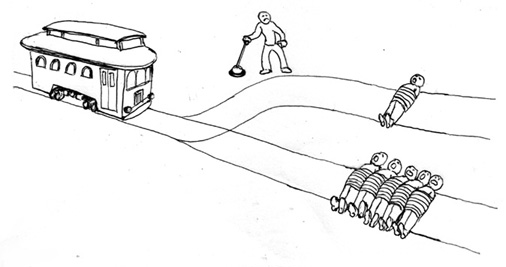
\includegraphics[width=0.7\linewidth]{img/trolley}
	\caption{The Trolley Problem \citep{Foot1967}. Illustration by \href{http://subcortex.com/}{Jesse J. Prinz}.}
	\label{fig:trolley}
\end{figure}

In the first few weeks of my Ph.D., I observed that layman interlocutors, when confronted with this question on the occasion of a social dinner, have a general tendency to conjure up disaster scenarios involving imminent accidents with unavoidable casualties. This reflex is likely to stem from the popularisation of the Trolley Problem \citep{Foot1967}, a famous thought experiment in moral philosophy, depicted in \Cref{fig:trolley}, in which a runaway trolley is headed straight toward five people tied up on the main track and unable to move. When pulled, a lever switches the trolley to a side track occupied by one person: what should you do? Answering this general question of what we \emph{ought} to do in any situation, what is a \emph{right} or \emph{wrong} decision, is the focus of the field of {normative ethics}. This dilemma illustrates a clash between two schools of thought: utilitarianism and deontological ethics. According to utilitarians, the rightfulness of an action should be evaluated based on its consequences, and actions maximising a \emph{utility} --the happiness and well-being for the affected individuals-- should be preferred. Conversely, deontologists evaluate the morality of actions \emph{per se}, according to a series of rules, rather than based on their consequences. Although this problem was initially introduced as a thought experiment, its transposition to the context of autonomous driving and arguably more realistic scenarios made it heavily cited in discussions regarding safety \citep[\eg][]{Lin2015,Bonnefon2016,Gogoll2017}. In early 2017, MIT's Media Lab launched the \emph{Moral Machine} platform \citep{Awad2018}, in which they invited members of the public to select the morally acceptable decision out of several options available to an autonomous vehicle. The authors argued that the recovered global preference would provide \emph{\enquote{essential topics to be considered by policymakers}}, and \citet{Noothigattu2018} proposed an implementation of a system aggregating these preferences, trained on the collected data. However, the relevance of this analogy to inform engineering and policy has been called into question. Thus, \citet{DeFreitas2019} point out that such dilemmas are unlikely to occur on real roads, hard to detect by perception systems and to act upon by control systems, and that they are distracting researchers from the more appropriate goal of how to avoid accidents altogether. Indeed, when we drive, we seldom find ourselves in such extreme situations but rather constantly ponder over less tragic considerations: Where does this vehicle intend to go? Do I have the time to proceed or should I yield? What is the appropriate speed to drive at right now? 
% https://www.grammarphobia.com/blog/2019/08/series-of-questions.html
The object of this thesis is to artificially reproduce this cognitive process of how to avoid accidents while driving, which is more a technical matter than an ethical one. Still, the Trolley Problem, though unrealistic, reveals and raises a number of legitimate questions. Should we base driving decisions on a set of rules? Can these rules be learned, \eg by imitating human drivers? Should we instead make decisions by comparing the utility of possible outcomes, like utilitarians advocate? And if so, how do we choose a good utility? This last interrogation becomes particularly sensitive if we add uncertainty to the Trolley Problem. Facing a potential collision, driving slowly decreases the risk of accident at the expense of efficiency, which can ultimately have an economical impact. What is the \emph{right} level of caution to take? This question directly translates as that of the \emph{value of life}, which has been taken up by economists for decades \citep{Abraham1960,Dreze1962,Schelling1968life,Banzhaf2014,Tirole2017,Charpentier2019} and has countless practical implications for public policies, including recent debates on lowering the speed limits on highways and trunk roads, but also on the appropriate lockdown durations during a pandemic.
It would be illusory to pretend that the practical implications of the Trolley Problem can simply be swept aside and entirely replaced by technicality. Throughout this manuscript, we will see that ethical concerns still underpin most assumptions and design choices of safety-critical software.


\subsection{Nuts and bolts of self-driving software}
\label{sec:nuts-and-bolts}

\begin{figure}[th]
	\centering
	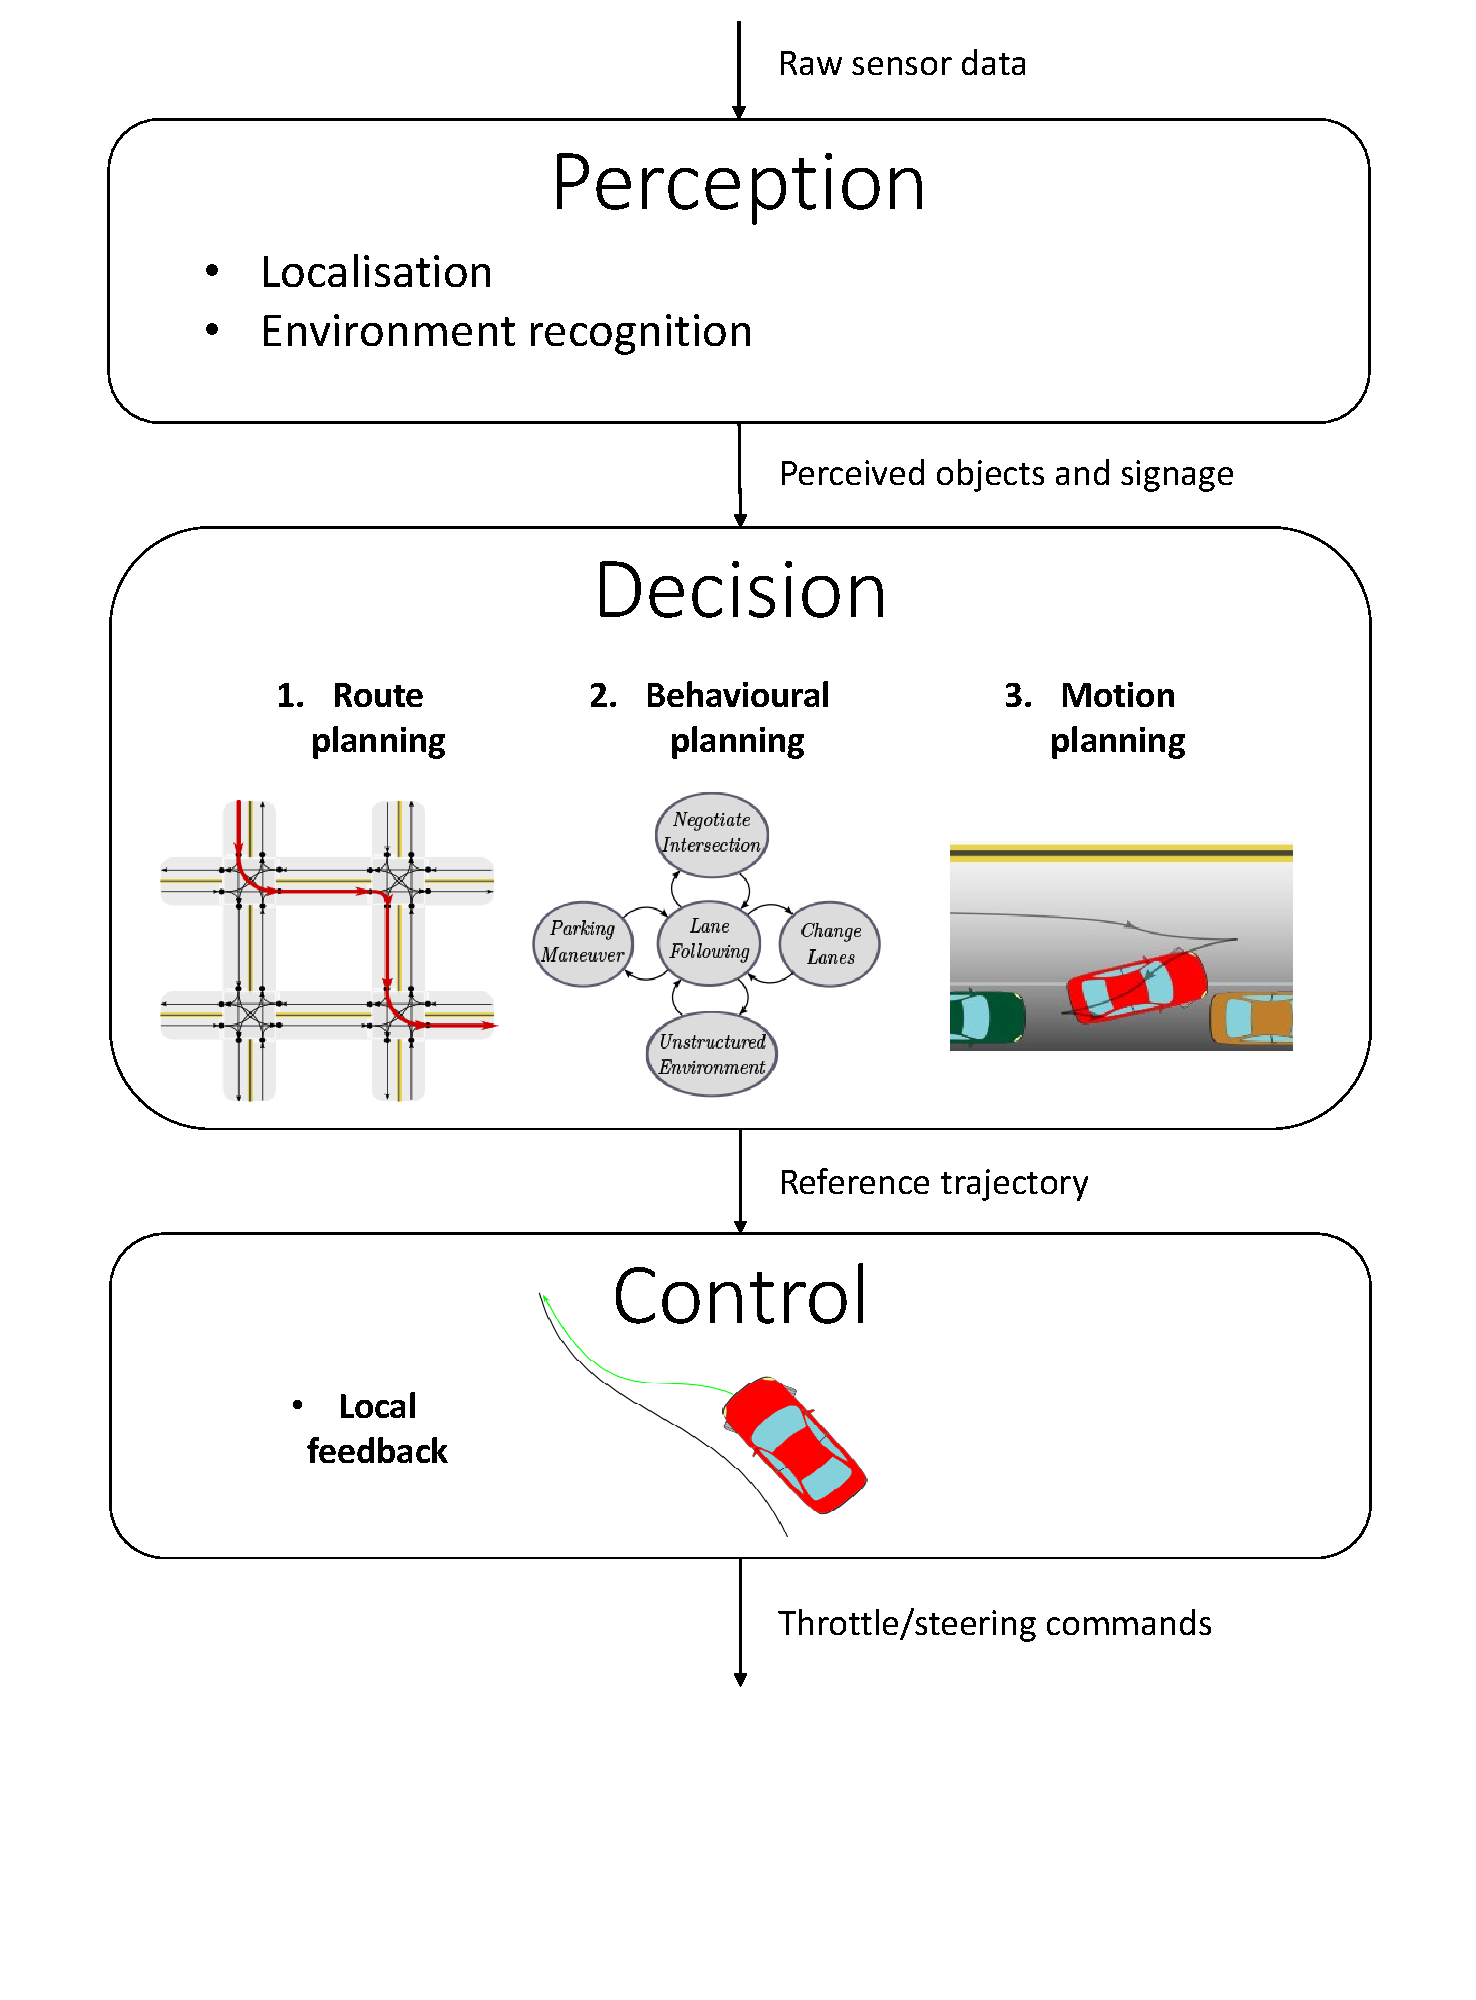
\includegraphics[trim={0 5cm 0 0}, clip, width=0.7\linewidth]{img/pipeline}
	\caption{The architecture of a typical self-driving software}
	\label{fig:robotics-pipeline}
\end{figure}

Historically, autonomous vehicles have been developed following a traditional robotics pipeline, illustrated in \Cref{fig:robotics-pipeline}. This architecture decomposes the task of driving as a series of three functions: \emph{Perception}, \emph{Decision}, and \emph{Control} (also called the Sense-Plan-Act paradigm, or Navigation, Guidance and Control in aerospace engineering). The {Perception} module takes raw sensor data as input and produces a high-level reconstruction of the scene. The {Decision} module then determines the desired trajectory of the vehicle, based on the current situation. Finally, the {Control} module manipulates forces, by way of steering and throttle controls, to track the desired trajectory. In the context of Autonomous Driving, the Decision module is often implemented with a hierarchical structure whose layers work at different timescales. First, a \emph{Route Planning} layer searches for the shortest route in a road network from the current location to the desired destination. Second, the \emph{Behavioural Planning} layer specifies a coarse driving behaviour through short-term goals or semantic decisions, such as changing lane, slowing down at an intersection, or yielding to a vehicle. This layer is thus responsible for following the planned route while adapting to the current state of the traffic in real-time. Third, the \emph{Motion Planning} layer generates a continuous, feasible trajectory that implements the desired behaviour while ensuring comfort and safety.

Great strides have been made in the two end-of-pipe tasks: Perception has benefited from the substantial progress in the field of computer vision due to the recent advent of deep learning \citep[surveyed in][]{janai2017computer}, and many Control schemes \citep[surveyed in][]{Polack2018} have been developed for ground vehicles. In the Decision module, Route Planning is virtually solved and already provided by services such as \href{https://wiki.openstreetmap.org/wiki/Routing}{Open Street Maps}, and there exist a vast body of Motion Planning algorithms, discussed in \Cref{chapter:2}. All these building blocks are widely used for industrial applications, including \gls{ADAS} functions such as \gls{LKA}, \gls{ACC}, \gls{AEB} or \gls{AES}; and in academic research challenges. Ultimately, we claim that Behavioural Planning remains the only neglected link in the chain. Indeed, most of these applications focused so far on simple settings with little complexity: \gls{ADAS} systems are mostly tailored for highway driving and struggle whenever required to interact with other drivers, \eg for merging into traffic\footnote{This difficulty, which motivated this thesis, was reported by engineers from the \gls{ADAS} team at Renault.}.
Similarly, most academic challenges focused on highway driving, with the exception of the DARPA Urban Challenge, which required more advanced interactions with other vehicles. Nevertheless, even this event still constituted a controlled environment, simple enough that all participants could rely on rule-based systems for behavioural planning \citep{Buehler2009}, such as finite state machines whose transitions are triggered by handcrafted criteria \citep[\eg][]{Baker2008}. Unfortunately, there is little hope that this approach can scale to complex scenes since responses tailored for specific use-cases cannot be easily merged. %TODO: ref needed

\subsection{Scope and Challenges of this Thesis}
\label{sec:scopes-and-challenges}

In the light of the above, this thesis is dedicated to addressing a weak link in the \gls{AD} chain: \emph{Behavioural Planning}.  We ask the following question: assuming that we had access to a ground truth perception and a perfectly accurate control system, what steps would remain to achieve fully autonomous driving?


\paragraph{Humans in the loop}

Unless restrained to dedicated infrastructure, Autonomous Vehicles will have to share the road with human drivers. This introduces a great deal of uncertainty in the decision problem. Indeed, while the location and velocity of a vehicle can be perceived, the mind of its driver remains impenetrable. Even though the present state is known, the future becomes uncertain: where are they headed? Are they paying attention to their surroundings? In that regard, it seems impossible to manually model all the factors involved in the human decision-making process. However, human drivers do not drive erratically either, and their behaviour is highly structured: humans drivers tend to follow the lanes, avoid collisions with other vehicles, and generally respect road signage. In other words, human drivers are \emph{predictable}. This motivates the idea of learning from data, and hope for a better comprehensiveness than handcrafted decision systems.%, either direct predictive models of human behaviours or a driving policy based on implicit predictions of what they might do next.
% We want to quantify uncertainty
% Recall aletoric vs epistemic uncertainty?

\paragraph{Learning to act}

The skill of driving a car involves taking a series of decisions, where early stages influence the resulting outcomes and subsequent reasoning at late stages. This aspect is known as sequential (or multistage) decision-making. Let us start by introducing some useful notations. At each time step $t$, the system is described by its \emph{state} $s_t$ that belongs to a measurable\footnote{A measurable space is a set with a $\sigma$-algebra, that allows to define random variables. For example, this set can finite ($[N]$), countable ($\Natural$), or continuous ($\Real$).} state space $\cS$. Then, the agent can take an \emph{action} $a_t$ within a measurable action space $\cA$, before transitioning to a next state $s_{t+1}\in\cS$, drawn from a conditional distribution $\Ps\parentheses{s_{t+1} \mid s_t, a_t}$ that we call the \emph{system dynamics} $\Ps\in\cM(\cS)^{\cS\times\cA}$, where $\cM(\cX)$ denotes the set of probability measures of a measurable set $\cX$. The agent actions can themselves be drawn from a distribution $\policy\parentheses{a_t\mid s_t}$, called the \emph{policy} $\policy\in\cM(\cA)^{\cS}$.

\gls{RL} is a general framework for learning-based sequential decision-making. It is formulated as an optimal control problem: the policy $\policy$ is chosen to maximise an objective function. It is generally formalised as a \gls{MDP}, \ie a tuple $(\gls+{cS}, \gls+{cA}, \gls+{transition}, \R, \discount)$ in which at each step $t$, the agent receives a bounded reward $R(s_t, a_t)$, where $R\in[0, 1]^{\cS\times\cA}$ is a deterministic reward function and $\discount\in[0,1)$ is a discount factor. Adequate long-term behaviour of policies $\policy$ is fostered by considering their \emph{return}.

\begin{definition}[Policy return]
	\begin{leftbar}[defnbar]
	The {return} $\return^{\gls+{policy}}$ of a policy $\policy$ is a random variable defined as the discounted sum of rewards 
	\begin{equation*}
	\gls+{return}^{\gls+{policy}} = \sum_{t=0}^\infty \discount^t \R(s_t, a_t)
	\end{equation*}
	accumulated along a trajectory $\tau = (s_0, a_0, s_1, a_1, \dots)$ induced by the policy $a_t\sim \policy(a_t|s_t)$ and system dynamics $s_{t+1}\sim \Ps(s_{t+1} \mid s_t, a_t)$.
	\end{leftbar}
\end{definition}

The performance of a policy $\policy$ is then evaluated through its \emph{value} function. 
\begin{definition}[Value functions]
	\begin{leftbar}[defnbar]
	\label{def:value-functions}
	The state value $\V^\policy(s)$ of a policy $\policy$ is the expected return of the policy when starting in a state $s$
	\begin{align*}
	\gls+{V}^\policy(s) \eqdef \expectedvalue\left[ \return^\policy \mid s_0=s\right].
	\end{align*}
	Similarly, the state-action value $\Q^\policy(s, a)$ of a policy $\policy$ is the expected return of the policy when starting in the state $s$ and taking the action $a$
	\begin{align*}
	\gls+{Q}^\policy(s, a) &\eqdef \expectedvalue\left[ \return^\policy \mid s_0=s, a_0 = a\right].
	\end{align*}
	\end{leftbar}
\end{definition}

This allows to define the goal of \glsxtrlong{RL}: finding an \emph{optimal} policy $\optimalpolicy$.

\begin{definition}[Optimality]
	\begin{leftbar}[defnbar]
	\label{def:optimality}
	A policy $\gls+{optimalpolicy}$ is said to be optimal if it maximises the value functions $V^\policy$ and $Q^\policy$ in every state and action.
	We also define the optimal value functions $\gls+{V}^\star$ and $\gls+{Q}^\star$ as 
	\begin{align*}
	&\forall s\in \cS, & \gls+{V}^\star(s) &\eqdef Q^{\policy^\star}(s) = \max_\policy V^\policy(s);\\
	&\forall (s,a)\in \cS\times\cA,& \gls+{Q}^\star(s, a) &\eqdef Q^{\policy^\star}(s, a) = \max_\policy Q^\policy(s, a).
	\end{align*}
	\end{leftbar}
\end{definition}

\paragraph{Sample efficiency}
Several performance measures have been introduced to evaluate \gls{RL} algorithms. In this thesis, we consider the goal of finding a near-optimal policy as fast as possible. The \emph{fixed-confidence} setting evaluates the smallest sample complexity, \ie number of interactions, required to find a near-optimal policy $\optimalpolicy$ with high probability. Alternatively, in the \emph{fixed-budget} setting, the \emph{simple regret} $\regret$ of an algorithm measures the \emph{expected} sub-optimality of the recommended policy $\hat{\policy}_n$ after a fixed number $n$ of interactions
\begin{equation*}
\gls+{regret}(s) \eqdef \expectedvalue_{\hat{\policy}_n} \left[ V^\star(s) - V^{\hat{\policy}_n}(s) \right].
\end{equation*}

%Conversely, in real environments where exploration is costly, another objective is to minimise the \textit{cumulative regret}.
%\begin{equation*}
%\cR_n(s_0, \cA) = \expectedvalue_{\hat{\policy}_t\sim \cA}\left[ \sum_{t=0}^{n-1} V^\star(s_t) - V^{\hat{\policy}_t}(s_t) \right]
%\end{equation*}

The goal of this thesis is to provide \emph{sample-efficient} algorithms for learning a driving policy. In the particular context of Behavioural Planning for Autonomous Driving, this goal will be articulated around a few main questions and challenges.

\paragraph{Model-free \vs model-based}

\glsxtrlong{RL} algorithms can be grouped into two main families. 
To find an optimal policy $\optimalpolicy$, model-based \glsxtrlong{RL} algorithms first attempt to estimate the \gls{MDP} parameters $\hat{P}$ and $\hat{R}$ based on a history of transitions $\cD = \{(s_{t},a_t, r_t, s_{t+1})\}$, using for instance \gls{MLE} in a hypothesis class of dynamics and reward functions:
\begin{equation*}
\max_{\hat{P}} \prod_{t}\hat{P}\parentheses{s_{t+1} \mid s_t,a_t} \quad \text{and} \quad \min_{\hat{R}} \sum_{t}\|R(s_t,a_t) - \hat{R}(s_t,a_t)\|^2_2.
\end{equation*}
This allows to \emph{plan} in the estimated \gls{MDP} $(\cS,\cA, \hat{P}, \hat{R}, \discount)$, \ie compute the associated optimal policy $\hat{\policy}^\star$. This can be achieved using planning algorithms such as Dynamic Programming or Linear Programming.
Conversely, model-free \gls{RL} algorithms do not estimate the underlying \gls{MDP} and aim instead to optimise a policy $\policy$ directly. Policy-based methods evaluate the value $Q^\policy$ of the current policy $\policy$, so that it can be locally improved \eg by gradient ascent. Value-based method bypass this alternation of evaluation and improvement steps by directly learning the optimal value function $Q^\star$.

The question of which approach is appropriate depends on the underlying problem. Indeed, model-based techniques are relevant when the dynamics are simple but the optimal policy is complex. For instance, the case of Computer Go was tackled in AlphaGo \citep{Silver2016,Silver2017,Silver2018} with a \gls{MCTS} planning module, which leveraged the knowledge of the Go dynamics (placing pawns on the board) to sample sequences of plies in a game tree. On the contrary, the model-free approach is useful when the system dynamics are complex, but the optimal policy is simple. Thus, a swimming robot would require massive fluid dynamics simulation to accurately predict the effect of moving its fins, while a simple periodic gait could suffice to propel it forward in the water. Which brings us to the question: which scenario does \gls{AD} fall into? Unfortunately, the answer is not so clear-cut. On the one hand, the motion planning literature has historically been heavily relying on kinematics and dynamics models to plan trajectories, as detailed in \Cref{chapter:2}. Reliable priors are available to describe the physics of a vehicle, but not so much for the actual driving policy. On the other hand, automotive companies such as Mobileye reportedly\footnote{These comments are reported from discussions between Renault and Mobileye.} advocated that the task of predicting a driving scene is actually more difficult than that of driving. In fact, the case of \glsxtrlong{AD} is peculiar in that the two problems of prediction and control are somewhat equivalent, due to the presence of other drivers: a good trajectory predictor can be used to predict the action that a human would take in place of the ego-vehicle, and a good driving policy can be applied to each agent in the scene to produce reasonable predictions of their trajectory. Hence, both approaches seem equally relevant and will be considered in this thesis.

\paragraph{Social interactions and coupled dynamics}

To ensure safety while driving, traditional motion planning techniques rely on conservative independence assumptions on the behaviour of other vehicles. This makes them suffer from an effect colloquially known as the \emph{\enquote{freezing robot problem}} \citep{Trautman2010}: due to massive uncertainty, these systems tend to struggle in situations that require interacting --or negotiating-- with other vehicles, such as unprotected left-turns, intersections, or highway merges (see \eg these \href{https://www.youtube.com/watch?v=HjtiiGCe1pE}{two} \href{https://twitter.com/nitguptaa/status/990683818825736192}{videos} where a Waymo car fails to merge). 
Thus, for an autonomous vehicle to efficiently integrate with the traffic flow, it must anticipate the effect of its own actions on the behaviour of other agents. This skill is known as \emph{socially-aware} decision-making. Unfortunately, interactions between vehicles translate into complex and coupled traffic dynamics where local deviations must be propagated from one vehicle to the next, which can result in a quick and chaotic build-up of uncertainty. We will need to contain this escalation to prevent instability in our predictions.

\paragraph{Ensuring safety}

The complexity of the task of driving leads us to consider learning algorithms. However, these methods typically raise a legitimate concern among car manufacturers: how can we guarantee the \emph{safety} of such systems, in the presence of uncertainty? In this thesis, we will strive to formalise this concern by formulating different notions of \emph{risk}, as functions of the distribution of outcomes induced by a policy. We will study \emph{Safe} \glsxtrlong{RL} algorithms, that seek to explicitly estimate and control the level of risk taken by a policy.

\paragraph{Balancing safety and efficiency}
However, protecting against risk often comes at the price of efficiency in achieving a goal.
Consider for a moment a situation where a vehicle is driving slowly in front of you on the road, and so you decide to overtake them. How do you know, at that very moment, that the driver has seen you and is not going to change lane at the last moment, causing an accident? In fact, you don't, at least not with certainty. In this situation, the only way to guarantee safety is to refrain from overtaking. By pushing this simple argument through to its conclusion, it becomes apparent that the only way to \emph{fully} ensure safety is to stay in the garage.
You are thus facing an irreducible dilemma: the two objectives of driving fast and safely are contradictory.
This opposition induces a trade-off that we typically observe with human drivers, especially in situations of negotiations: some people adopt \emph{aggressive} behaviours and try to force their way through traffic, while others act more \emph{defensively}, favouring safety. This ambiguity is difficult to capture manually in an objective function and soon leads to the pitfall of reward engineering. To provide a principled control over this trade-off, the learning algorithms that we consider will be required to respect an \emph{adjustable} level of risk.

\section{Outline and Contributions}

\begin{figure}[ht]
	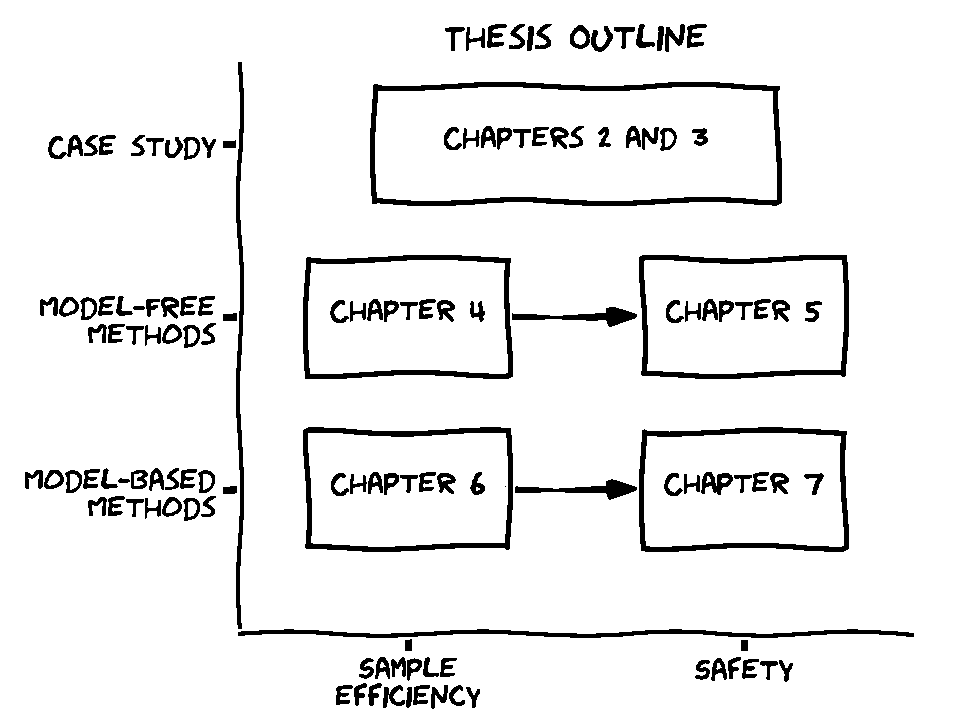
\includegraphics[width=0.9\linewidth]{img/outline}
	\caption{This thesis is structured around two disjunctions: model-free \vs model-based on the one hand, and sample-efficiency \vs safety on the other hand.}
	\label{fig:thesis-outline}
\end{figure}

% Part I
The ultimate goal of this thesis could be summarised in the following question: \emph{\enquote{how can an algorithm learn to drive and avoid accidents?}}. The first step in such an endeavour must necessarily be to formalise more precisely the meaning of this ill-posed formula, which we try to do in \textbf{\Cref{part:1}}.
It is only natural that we begin this effort by turning to the standard model for sequential decision making: the \glsxtrlong{MDP}. At first glance, this framework shines with its simplicity and elegance, but also its apparent generality and representation power. Yet, as we embark on the ambitious task of casting the blurry problem of autonomous driving into this rigid mould, we highlight in \textbf{\Cref{chapter:2}} how reductive each step of the formalisation is, how approximations and assumptions always hide behind each symbol and each equation. This observation is supported by the numerous variations of the framework developed by the research community, in as many attempts to address these concerns. Such limitations are as varied as partial observability, temporal abstraction, the reward hypothesis, transfer from simulation to real-world and safety; and we relate these research directions to specific works in the autonomous driving literature.

In order to progress, we put aside some of these questions in \textbf{\Cref{chapter:3}} and commit to an (observable) state space, a (hierarchical) action space, a (quasi-linear) system dynamics and a (dense) reward function that we deem suitable for a large class of behavioural planning tasks. This allows us to refocus on two fundamental issues: \textit{sample-efficient} and \textit{safe} \glsxtrlong{RL}. In the sequel we tackle them through the perspective of the two main approaches to \glsxtrlong{RL} aforementioned: first model-free, and then model-based algorithms. This organisation is depicted in \Cref{fig:thesis-outline}.

% Part II
\textbf{\Cref{part:2}} is dedicated to the study of how model-free methods can be applied for efficient and safe \glsxtrlong{AD}. In \textbf{\Cref{chapter:4}}, we question the choice of state representation and model architecture in relation to their associated sample-efficiency. In particular, we identify desirable properties and inductive biases that the policy should enjoy, such as \emph{permutation invariance} with respect to vehicles in the scene. We propose an attention-based architecture that fulfils our criteria, and compare it to standard representations and model architectures that have been used for behavioural planning tasks. 

In \textbf{\Cref{chapter:5}}, we consider a continuous notion of risk, defined as an expected discounted sum of a cost signal. This formulation allows highlighting  a trade-off between two separate objectives: the traditional return associated with task completion, and the risk related to safety. In this multi-objective perspective, the Pareto frontier of non-dominated policies defines a spectrum of behaviours, from risk-averse on one side to risk-seeking on the other. In order to explicitly control the level of risk taken in real-time, we place ourselves within the \gls{BMDP} framework, in which the risk is constrained to lie below an --adjustable-- threshold. 
So far, \glspl{BMDP} could only be solved in the case of finite state spaces with known dynamics. This chapter extends the state-of-the-art to environments with continuous state space and unknown dynamics. We show that the solution to a \gls{BMDP} is a fixed point of a novel Budgeted Bellman Optimality operator, which enables to estimate both the expected return and risk of an action, in a model-free fashion. This observation allows us to introduce natural extensions of Deep Reinforcement Learning algorithms to address large-scale \glspl{BMDP}.

% Part III
\textbf{\Cref{part:3}} is devoted to the study of model-based methods, that solve the \glsxtrlong{RL} problem by planning with a learned generative model.
In \textbf{\Cref{chapter:6}}, we assume that a reliable generative model has already been learnt and focus on the sample-efficiency of the planning procedure specifically. More precisely, we look into the theoretical and practical aspects of planning algorithms under budget constraints. First, we consider the \gls{OLOP} algorithm that enjoys good theoretical guarantees but is overly conservative in practice, as we show in numerical experiments. We propose a modified version of the algorithm with tighter upper-confidence bounds, \KLOLOP, that leads to better practical performances while retaining the sample complexity bound. Second, we study a limitation of \gls{MCTS} algorithms: they do not identify together two similar states reached via different trajectories and represented in separate branches of the tree. We propose a \emph{graph-based} planning algorithm, which takes into account this state similarity, provide a regret bound that depends on an improved problem-dependent measure of difficulty, and illustrate its empirical benefits numerically.

In \textbf{\Cref{chapter:7}}, we look back into the issue of \emph{model bias}, which refers to the gap that exists between a learned model and the true system dynamics, and can dramatically degrade the performance of the planned trajectory. More specifically, we study the problem of \emph{robust} and \emph{adaptive} \gls{MPC} of a linear system, with unknown parameters that are learned along the way (adaptive), in a critical setting where failures must be prevented (robust).
To that end, instead of merely considering a point estimate of the dynamics, we leverage non-asymptotic linear regression to build an entire \emph{confidence region} that contains the true dynamics with high probability.
To effectively propagate this parametric uncertainty, we design a predictor that produces a tight interval hull bounding the system trajectories. Having observed the instability of traditional interval predictor techniques, we propose a new one whose stability is guaranteed by a Lyapunov function analysis and verification of linear matrix inequalities.
These tools enable us to guarantee the system stabilisation and robust constraint satisfaction, through an \gls{MPC} algorithm based on a stabilising control that uses the predicted interval.
Finally, in order to go beyond stabilisation problems only, we tackle the minimax control of more general (non-convex) costs that naturally arise in many practical problems. To that end, we combine our results with the tree-based planning techniques of \Cref{chapter:6}. By adapting the theoretical guarantees at each layer, we provide the first end-to-end regret analysis for this setting. Interestingly, our analysis naturally adapts to handle multiple models and combines with a data-driven robust model selection strategy, which enables to relax the modelling assumptions. We strive to preserve tractability at any stage of the method, that we illustrate numerically.

%!TEX root = ../PhD_thesis__Edouard_Leurent

\subsection*{List of publications}

\subsubsection*{Publications in international conferences with proceedings}

\begin{itemize}
	\item \fullcite{Leurent2020beyond} (used in \Cref{chapter:7})
	\item \fullcite{Leurent2020monte} (used in \Cref{chapter:6})
	\item \fullcite{Leurent2020robust} (used in \Cref{chapter:7})
	\item \fullcite{CarraraLeurent2019} (used in \Cref{chapter:5})
	\item \fullcite{Leurent2019interval} (used in \Cref{chapter:7})
	\item \fullcite{Leurent2020practical} (used in \Cref{chapter:6})
\end{itemize}

\subsubsection*{Workshop presentations in international conferences}

\begin{itemize}
	\item \fullcite{Leurent2019social} (used in \Cref{chapter:4})
	\item \fullcite{Leurent2018approximate} (used in \Cref{chapter:7})
\end{itemize}

\subsubsection*{Software}

\begin{itemize}
	\item \fullcite{highway-env} (used in \Cref{chapter:3,chapter:4,chapter:5,chapter:6,chapter:7})
\end{itemize}

\subsubsection*{Collaborations not presented in this thesis}

\begin{itemize}
	\item \fullcite{Menard2020Fast}
	\item \fullcite{Kaufmann2020adaptive}
	\item \fullcite{Jonsson2020planning}
\end{itemize}

\chapter{Introduction}

\begin{flushright}
	\begin{tabular}{@{}l@{}}
		\emph{Pour soulever un poids si lourd,}\\
		\emph{Sisyphe, il faudrait ton courage !}\\
		\emph{Bien qu’on ait du cœur à l’ouvrage,}\\
		\emph{L’Art est long et le Temps est court.}\\
	\end{tabular}
	
	Charles Baudelaire, \href{https://eleurent.github.io/sisyphe/texts/le-guignon.html}{\emph{Le guignon}}.
\end{flushright}

\section{Context and scope}
\section{Our contributions}
\section{Outline}
\section{List of publications}
\part{Case Study: Learning to Drive}
\chapter{Problem statement}
\section{Sequential decision-making}
\subsection*{Motion Planning}
\subsection*{Imitation Learning}
\subsection*{Reinforcement Learning}
\section{States and partial observability}
\section{Actions and temporal abstraction}
\section{Rewards and inverse reinforcement learning}
\section{Traffic dynamics}
\chapter{The \texttt{highway-env} software}
\part{Model-free}
\chapter{Understanding Social Interactions}
\section{Common state representations}
\section{A social attention architecture}
\chapter{Acting under Adjustable Constraints}
\section{Budgeted dynamic programming}
\section{Budgeted reinforcement learning}
\part{Model-based}
\chapter{Planning Fast}
\begin{flushright}
	\begin{tabular}{@{}l@{}}
		\emph{Nous voulons, tant ce feu nous brûle le cerveau,}\\
		\emph{Plonger au fond du gouffre, Enfer ou Ciel, qu’importe ?}\\
		\emph{Au fond de l’Inconnu pour trouver du nouveau !}\\
	\end{tabular}

	Charles Baudelaire, \href{https://eleurent.github.io/sisyphe/texts/le-voyage.html}{\emph{Le voyage}}.
\end{flushright}

\section{Open-loop optimistic planning}
\section{State-aware planning}
\chapter{Preparing for the Worst}

\begin{flushright}
	\begin{tabular}{@{}l@{}}
		\emph{Two roads diverges in a wood, and I--}\\
		\emph{I took the one less traveled by,}\\
		\emph{And that has made all the difference.}\\
	\end{tabular}

	Robert Frost, \href{https://eleurent.github.io/sisyphe/texts/the-road-not-taken.html}{\emph{The Road Not Taken}}.
\end{flushright}


\section{Confident model estimation}
\section{State interval prediction}
\section{Robust control and constraint satisfaction}

%!TEX root = ../../PhD_thesis__Edouard_Leurent.tex

\makeatletter
\def\toclevel@chapter{-1}
\makeatother

%TODO: Discussion ?
\chapter{General Conclusion and Perspectives}
\label{chapter:conclusion}

\begin{flushright}
	\begin{tabular}{@{}l@{}}
		\emph{Nos équipiers}\\
		\emph{\hspace*{1.0cm}Sur les voies}\\
		\emph{\hspace*{0.5cm}Ralentissez}\\
	\end{tabular}

	Vinci Autoroutes\footnote{Writings collected by \href{https://twitter.com/pooredward/status/1273249408231124994}
		{@pooredward}.}\hspace*{1cm}
\end{flushright}

\section{Conclusion on our contributions}
In this thesis, we proposed a learning-based approach to the problem of behavioural planning for autonomous vehicles, with a focus on situations where several drivers are interacting. Following an in-breadth (\Cref{chapter:2}) as well as in-depth (\Cref{chapter:3}) initial investigation, we identified a set of key issues which make this problem challenging. We now recall each of these subjects, and precise how we strived to address them both in the model-free approach of \Cref{part:2} and the model-based approach of \Cref{part:3}.

%TODO highlight our most significant contributions

\paragraph{Coupled social dynamics}
In dense traffic, the dynamics of distinct vehicles are locally coupled, due to how drivers react and adapt to their surroundings. Consequently, predicting the course or acting in a driving scene requires a \emph{social awareness} skill: the ability to accurately understand and exploit these couplings.
In \Cref{chapter:4}, this skill was implemented through a \emph{social attention} mechanism in the policy architecture, which enables the agent to filter out irrelevant objects from a complex driving scene and retain only those that represent a risk of collision. In \Cref{chapter:5}, this coupling was made even more implicit by describing the motion of a vehicle $i$ through a dynamical model $\dot{x_i} = f_i(x)$ hat accepts the whole traffic state $x$ as an input.

\paragraph{Uncertainty due to human drivers}
Another key difficulty lies in the uncertainty of human behaviours. In \gls{RL}, the traditional approach to account for uncertainty is to incorporate stochasticity in the system dynamics, as we did in \Cref{chapter:5} where the objectives are formulated in terms of \emph{expected} rewards and costs. Incidentally, we also observed in \Cref{chapter:4} that our attention-based architecture is highly sensitive to ambiguous and disambiguated information, such as vehicles' destinations. In \Cref{chapter:7} however, we adopted another view and assumed that the dynamics were (close to) deterministic, but dependent on some unknown parameters --both continuous and discrete-- that could be estimated along the way.

\paragraph{Safety}
To deal with this uncertainty, three models of safety have been studied. In \Cref{chapter:5}, following the \gls{CMDP} framework, we formalised risk as the expected discounted sum of an additional cost signal $\constraint(s,a)$ --separate from the rewards $\reward(s,a)$-- constrained to remain below a threshold $\budget$. In \Cref{chapter:7}, we introduced a novel interval predictor allowing us to bound the set of reachable trajectories given the current parametric uncertainty over dynamics. This enabled us to cast safety as a robust stabilisation and constraint satisfaction problem, ensuring that the systems stays at all time within a safe space $\safestates\times\safecontrols$. Finally, to go beyond stabilisation problems, we considered a third formalisation of safety as a worst-case outcome, and proposed an algorithm for the minimax control of a generic reward function $\R(s,a)$.

\paragraph{Trade-off between safety and efficiency}
As we've just seen, safety is always defined with respect to some \emph{admissible} uncertainty. The larger the set of scenarios one is willing to consider and protect against, the more conservative they need to be to ensure safety. In particular, situations that require interacting with other agents are always susceptible to lead to accidents, when considering unlikely adversarial scenarios. In that sense, \emph{absolute safety is not achievable}, or only at the cost of usability. To strike the right level of safety, we need to consider the right level of uncertainty, the right set of outcomes. In \Cref{chapter:7}, the size of this ambiguity set to protect against can be controlled by adjusting the confidence level $\delta$ for continuous parameters (\eg driving style), and by adding or removing $(A,\phi)$-modelling assumptions from the multi-model extension, for discrete parameters (\eg potential destinations or lanes for a vehicle). In \Cref{chapter:5}, we embrace this trade-off even more explicitly. Rather than trying to adjust the scope and size of the uncertainty at its source, we instead directly control its effects on both the efficiency (rewards) of the policy and its safety (costs), by training a \emph{budgeted} policy $\budgetedpolicy$ that takes as input the desired level of risk $\confidence$.

\paragraph{Sample efficiency}
As for most reinforcement learning problems, we were concerned by minimising the number of samples required to reach optimality. To that end, we exploited the specificities and structures of the behavioural planning problem in several ways. In \Cref{chapter:4}, we embedded an inductive bias into the policy architecture by enforcing its invariance to permutations of the scene description, and observed that this fosters faster learning. In \Cref{chapter:7}, some structure was similarly imposed, on the dynamics model this time, in the form of a parametrised linear model which allowed to significantly reduce the dimension of the hypothesis space. We were also able to provide a bound on the simple regret relating the agent performance to the number of observed transition samples. In \Cref{chapter:6}, we looked into the sample efficiency of the planning procedure, and specifically tree-based planning algorithms. First, in the case of stochastic dynamics representing human behaviours, we proposed a modification of the \OLOP algorithm that improves its empirical sample complexity by an order on magnitude, while retaining its theoretical guarantees. Second, we showed that merging similar nodes in the lookahead tree enables to decrease the near-optimal branching factor featured in the regret bound of the algorithm. This translated as substantial empirical improvements in simple path planning tasks, where distinct sequences of actions lead to overlapping trajectories.


\section{Outstanding issues and perspectives}

In this section, I will adopt a more personal and subjective standpoint, and discuss which are the main barriers between research and industrialisation. Indeed, though we never intended for this thesis to lead directly to products, practical applications remains the long haul goal that motivates our work, and I must now examine our contributions again in this light.

A first and general concern of mine is that, beside the warm comfort of the well-behaved theoretical frameworks in which we place ourselves, the sheer complexity of the real world can be overwhelming. While any single aspect --partial observability, temporal abstraction, non-stationarity, risk aversion, you name it-- can be isolated and studied independently, the question of how to merge all these approaches into one single integrated product seems arduous, if not hopeless. Yet, any candidate algorithm not addressing any of these issues would be unfit.
In the sequel, I will not be so ambitious but reflect instead on a more reasonable question: are the methods that we developed likely to be suitable for a real-world application?

\paragraph{Reinforcement Learning in continuous states}

Let us start by our work in \Cref{part:2}. Following a model-free perspective in continuous states, we resorted function approximation using neural networks. Unfortunately, Deep Learning interacts with Reinforcement Learning algorithms in ways that are yet to be understood, but already infamous for their brittleness. In \Cref{chapter:4}, even our best policies after training still suffer a prohibitive rate of collisions of \SI{5}{\per}, considerably higher than the required performances. 
As we discussed, this may be attributed to the reward function that would not penalise collisions enough, but reward engineering is tedious and might in turn lead to over-conservative policies. The budgeted approaches of \Cref{chapter:5} were meant to address this issue, but at the price of an increased complexity, and our negative result of \Cref{thm:contraction} raises concerns over convergence in the general case. 
Another concern lies in our use of a very naive exploration policy --the $\epsilon$-greedy-- which takes random actions at a fixed frequency, a strategy widely considered as inefficient and damaging, yet which we had no choice but resorting to in the absence of a better solution. Guided exploration strategies tailored for regret minimisation, and especially following the \gls{OFU} principle, have been studied in the context of finite state-action spaces \citep{Auer2009,Azar2017}. 
These methods typically require the ability of counting the number of state visits, the question of how they can be extended to continuous spaces constitutes a promising research perspective. First steps have recently been made in that direction, by either relying on approximated \emph{pseudo-counts} \citep{Guyon2017}, or by deriving similar regret bounds under linear function approximation \citep{Jin2020}.

\paragraph{Trial without error?}

% In this thesis, we tried to solve behavioural planning in simulation, as a necessary step to solve it in real world. Thus treated simulation as our target task. 
Assume for a moment that the research community was able to solve the aforementioned problem and came up with exciting new algorithms for continuous state space with promising regret bounds. There remains an inevitable and fatal limitation: \emph{the foundations of \glsxtrlong{RL} are intrinsically based on trial and error}. Unfortunately, this is not an acceptable paradigm for the development of safety-critical problems such as \glsxtrlong{AD}. For reference, when we applied the model-free methods of \Cref{part:2} to very simple tasks, they converged in about 50k interaction samples, which represents about \SI{15}{\hour} of driving. Throughout training, the agents experienced about two thousand collisions. More generally, having vehicles \emph{exploring} on the roads among human drivers is morally inconceivable. Is there any chance at all to come up with learning algorithms that do not require actually causing accidents while training?

\paragraph{Safety guarantees}

As a first candidate, the line of work of Safe Control is committed to develop algorithms that are guaranteed never to reach an unsafe state, or with a provably bounded probability of failure. 
Likewise, in \Cref{chapter:7}, we managed to obtain some theoretical guarantees: a robust constraint satisfaction result, and a lower-bound on the worst-case outcome, that increases towards near-optimal performance with the number of samples. However, it is evident that these results are worth as much as their underlying assumptions, which could be: not much. Indeed, it seems very dubious that the complexity of human behaviours can be accurately described by our linear dynamics \Cref{assumpt:structure}, and our own proposed system largely overlooks large parts of the driving task. With \Cref{assumpt:feasible-constr}, the safe region $\safestates$ cannot be chosen freely, but must contain the basin of attraction $\safestates_{f}$ whose size grows with uncertainty. Finally, the assumptions of \Cref{thm:control-error} do not hold even in our simple simulations: the behaviours of observed vehicles are not persistently excited (\ie constantly braking before their leading vehicle and changing lanes). More generally, safety analyses can never protect against unmodeled events: a tree or a package falling down the road. Yet, having to model the world is daunting, especially since theoretical analysis imposes an additional constraint on the modelling effort, often at the expense of empirical performance. This may explain why practical achievements often precede their formal analysis. In the end, do we prefer relying on a simpler model that we can analyse under some assumptions unlikely to hold in practice, or more complex black-box models which tend to perform better on experimental benchmarks? Fortunately, all is not bleak and it has been observed in countless occasions that even when the guarantees do not hold, the founding principles of an algorithm can lead to designs that still exhibit the desired properties, and can robustly generalise. An example is the reliable of control systems in the aerospace industry, which even though aircraft dynamics are not \emph{really} linear and measurement noises are not \emph{really} Gaussian.

% TODO: still, current safety frameworks are not well suited to AD. Stabilisation: meh. Safe states: meh.
% Perspective: investigate new ones (which ?)
% But always the same problem: guaranteed protection against rare events = conservativeness.

\paragraph{Simulation and beyond?}

Another obvious way to avoid trial-and-error in the real world is to rely on simulation. Of course, the effort of modelling a complex world remains, but dropping the analysability requirement significantly relaxes the constraints on how this description can be expressed. We can safely expect that simulations will continue to play an increasingly significant part in \gls{AD} technologies, for both offline pre-training and online planning. This can be the occasion to divert our research efforts from the traditional regret minimisation objective, which does not make much sense in a simulated environments where rewards are free but samples are costly. In contrast, a promising research direction is the study of the more appropriate Pure Exploration setting, which aims at relating the policy suboptimality to the number of samples. I already took part in collaborations exploring this direction \citep{Jonsson2020planning,Kaufmann2020adaptive,Menard2020Fast} and hope to pursue this path further. 
Finally, relying on simulation introduces the additional question of how to adapt knowledge from simulation to the real world. A fine-tuning training process in real conditions would involve experiencing real failures again, though hopefully in reduced numbers, which could be realistic under human interventions \citep{Saunders2018,Kendall2019}. Another path of interest to me could be to leverage offline \gls{RL} methods \citep{Thomas2015,Laroche2019}, that could enable to safely improve pre-trained policies around nominal states in a dataset of real driving data.
